\section{Algoritmo di Hoshen-Kopelman}
L’algoritmo di Hoshen-Kopelman (HK76) è una tecnica di etichettatura multipla dei cluster. Il reticolo viene visitato sito per sito per colonne, partendo dallo spigolo in alto a sinistra per arrivare a quello in basso a destra. Si prenda, ad esempio, il reticolo
in figura
\begin{figure}[H]
	\centering
	\scriptsize % Riduce la dimensione del testo
	\setlength{\tabcolsep}{5.4pt} % Riduce lo spazio tra le colonne
	\renewcommand{\arraystretch}{1.3} % Riduce lo spazio verticale tra le righe
	\begin{minipage}{0.45\textwidth}
		\centering
		\begin{tabular}{|*{15}{c|}}
			\hline
			0 & 1 & 0 & 0 & 1 & 1 & 0 & 0 & 0 & 1 & 0 & 1 & 0 & 1 & 0 \\
			\hline
			0 & 1 & 1 & 0 & 0 & 0 & 1 & 0 & 0 & 1 & 1 & 1 & 1 & 1 & 1 \\
			\hline
			0 & 1 & 0 & 0 & 0 & 1 & 1 & 1 & 1 & 0 & 0 & 1 & 0 & 0 & 0 \\
			\hline
			1 & 0 & 1 & 0 & 1 & 0 & 1 & 0 & 0 & 0 & 1 & 0 & 0 & 0 & 0 \\
			\hline
			0 & 1 & 0 & 1 & 1 & 0 & 1 & 0 & 0 & 0 & 1 & 0 & 0 & 1 & 0 \\
			\hline
			0 & 0 & 1 & 1 & 1 & 1 & 1 & 0 & 1 & 1 & 1 & 1 & 1 & 0 & 1 \\
			\hline
			0 & 0 & 1 & 1 & 1 & 0 & 0 & 0 & 0 & 1 & 1 & 1 & 1 & 0 & 1 \\
			\hline
			0 & 1 & 0 & 1 & 1 & 1 & 1 & 0 & 1 & 1 & 1 & 1 & 0 & 1 & 0 \\
			\hline
			0 & 1 & 0 & 0 & 1 & 1 & 0 & 0 & 1 & 1 & 1 & 0 & 0 & 0 & 1 \\
			\hline
			1 & 0 & 0 & 0 & 0 & 0 & 0 & 0 & 1 & 0 & 0 & 0 & 0 & 1 & 0 \\
			\hline
			0 & 0 & 0 & 0 & 1 & 0 & 1 & 0 & 1 & 1 & 0 & 1 & 1 & 1 & 1 \\
			\hline
			1 & 1 & 0 & 0 & 0 & 1 & 0 & 1 & 0 & 1 & 1 & 1 & 1 & 1 & 1 \\
			\hline
			1 & 1 & 1 & 0 & 0 & 1 & 1 & 0 & 1 & 0 & 0 & 1 & 0 & 0 & 0 \\
			\hline
			0 & 1 & 0 & 1 & 0 & 1 & 1 & 1 & 0 & 1 & 0 & 0 & 0 & 1 & 1 \\
			\hline
			1 & 1 & 1 & 1 & 0 & 0 & 0 & 1 & 1 & 0 & 0 & 1 & 0 & 1 & 0 \\
			\hline
		\end{tabular}
	\end{minipage}
	\hfill
	\begin{minipage}{0.45\textwidth}
		\centering
		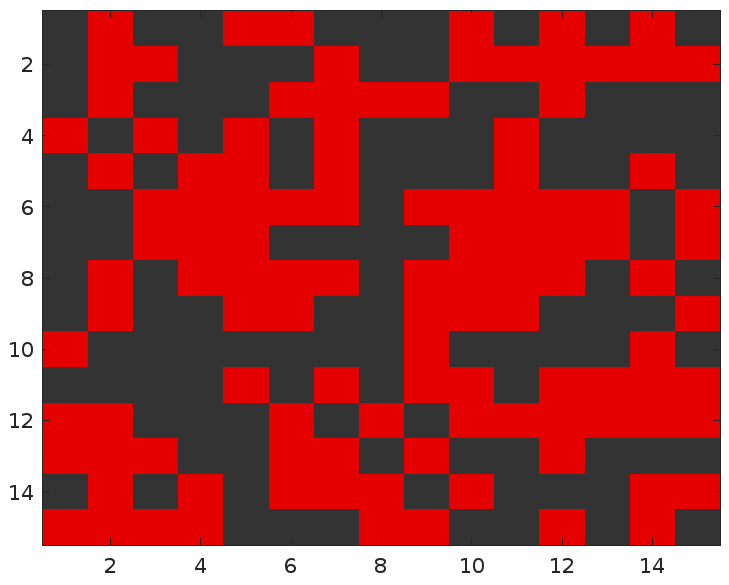
\includegraphics[width=\linewidth]{images/basegrid}
		\label{fig:basegrid}
	\end{minipage}
\end{figure}
\noindent
Durante la visita del reticolo, quando si incontra un sito occupato, allora: \textbf{(1)} Se il sito non è connesso ad altri siti occupato sopra o a sinistra, si inizia un nuovo cluster, a cui viene assegnata una \texttt{label} \textbf{(2)} Se c’è un primo vicino sopra o a sinistra occupato (uno solo dei due), il sito viene aggiunto al cluster del primo vicino occupato \textbf{(3)}Se i suoi primi vicini sono entrambi occupati, ma appartengono allo stesso cluster, il sito viene aggiunto al cluster dei primi vicini \textbf{(4)} Se i suoi primi vicini sono entrambi occupati, e non appartengono allo stesso cluster, il sito viene aggiunto al cluster con la \texttt{label} minore. Ad esempio, il cluster associati al reticolo precedente sono
mostrati in figura
\begin{figure}[H]
	\centering
	\scriptsize % Riduce la dimensione del testo
	\setlength{\tabcolsep}{3.5pt} % Riduce lo spazio tra le colonne
	\renewcommand{\arraystretch}{1.3} % Riduce lo spazio verticale tra le righe
	\begin{minipage}{0.4\textwidth}
		\centering
		\begin{center}
			\begin{tabular}{|*{15}{c|}}
				\hline
				0 & 1 & 0 & 0 & 2 & 2 & 0 & 0 & 0 & 3 & 0 & 4 & 0 & 5 & 0 \\
				\hline
				0 & 1 & 1 & 0 & 0 & 0 & 6 & 0 & 0 & 3 & 3 & 3 & 3 & 3 & 3 \\
				\hline
				0 & 1 & 0 & 0 & 0 & 7 & 6 & 6 & 6 & 0 & 0 & 3 & 0 & 0 & 0 \\
				\hline
				8 & 0 & 9 & 0 & 10 & 0 & 6 & 0 & 0 & 0 & 11 & 0 & 0 & 0 & 0 \\
				\hline
				0 & 12 & 0 & 13 & 10 & 0 & 6 & 0 & 0 & 0 & 11 & 0 & 0 & 14 & 0 \\
				\hline
				0 & 0 & 15 & 13 & 10 & 10 & 6 & 0 & 16 & 16 & 11 & 11 & 11 & 0 & 17 \\
				\hline
				0 & 0 & 15 & 13 & 10 & 0 & 0 & 0 & 0 & 16 & 11 & 11 & 11 & 0 & 17 \\
				\hline
				0 & 18 & 0 & 13 & 10 & 10 & 10 & 0 & 19 & 16 & 11 & 11 & 0 & 20 & 0 \\
				\hline
				0 & 18 & 0 & 0 & 10 & 10 & 0 & 0 & 19 & 16 & 11 & 0 & 0 & 0 & 21 \\
				\hline
				22 & 0 & 0 & 0 & 0 & 0 & 0 & 0 & 19 & 0 & 0 & 0 & 0 & 23 & 0 \\
				\hline
				0 & 0 & 0 & 0 & 24 & 0 & 25 & 0 & 19 & 19 & 0 & 26 & 26 & 23 & 23 \\
				\hline
				27 & 27 & 0 & 0 & 0 & 28 & 0 & 29 & 0 & 19 & 19 & 19 & 19 & 19 & 19 \\
				\hline
				27 & 27 & 27 & 0 & 0 & 28 & 28 & 0 & 30 & 0 & 0 & 19 & 0 & 0 & 0 \\
				\hline
				0 & 27 & 0 & 31 & 0 & 28 & 28 & 28 & 0 & 32 & 0 & 0 & 0 & 33 & 33 \\
				\hline
				34 & 27 & 27 & 27 & 0 & 0 & 0 & 28 & 28 & 0 & 0 & 35 & 0 & 33 & 0 \\
				\hline
			\end{tabular}
		\end{center}
	\end{minipage}
	\hfill
	\begin{minipage}{0.45\textwidth}
		\centering
		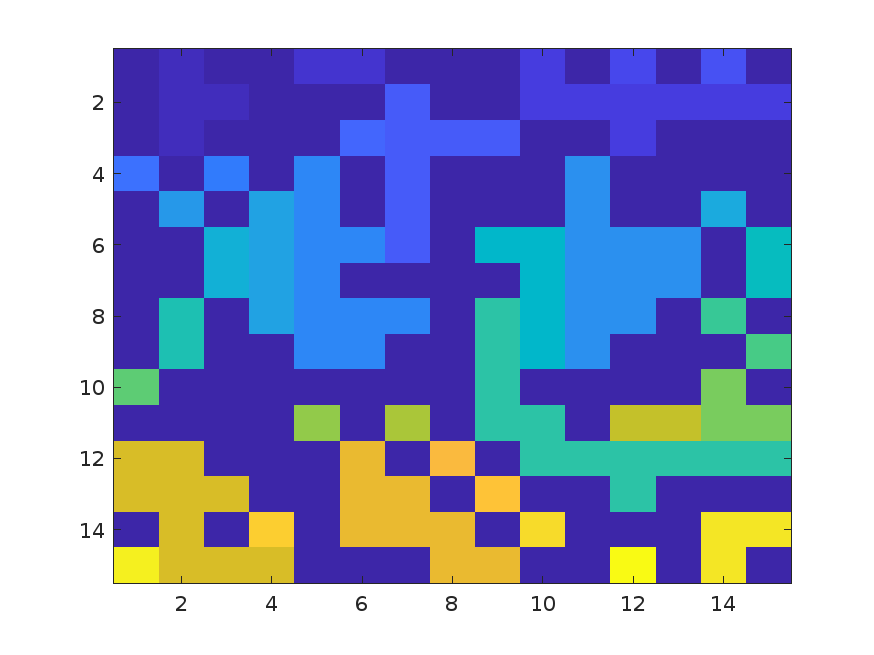
\includegraphics[width=\linewidth]{images/labels}
		\label{fig:basegrid}
	\end{minipage}
\end{figure}
\noindent
Tuttavia, quando si incontra un caso come quello descritto nel punto \textbf{(4)}, occorre  memorizzare che i due cluster sono in realtà lo stesso cluster. Questo viene fatto usando un vettore chiamato \textbf{Label of Label} (\texttt{LofL}), che contiene tutta l’informazione necessaria sui label dei cluster. In particolare: 
per un *good label*, memorizza la taglia del cluster; 
per *bad label*, memorizza qual è il vero cluster label a cui questo label appartiene.  Questa distinzione viene fatta attraverso i segni dei numeri interi contenuti in LofL. Di seguito è riportato il LofL corrispondete al reticolo preso in esame

\vspace{15px}
\noindent
\begin{tabular}{|c|*{12}{c|}}
	\hline
	\textbf{Label} & 1 & 2 & 3 & 4 & 5 & 6 & 7 & 8 & 9 & 10 & 11 & 12 \\
	\hline
	\textbf{Rank} & 4 & 2 & 10 & -3 & -3 & 24 & -6 & 1 & 1 & -6 & 33 & 1 \\
	\hline
\end{tabular}

\vspace{10px}
\noindent
\begin{tabular}{|c|*{12}{c|}}
	\hline
	\textbf{Label} & 13 & 14 & 15 & 16 & 17 & 18 & 19 & 20 & 21 & 22 & 23 & 24 \\
	\hline
	\textbf{Rank} & -10 & 1 & -10 & -11 & 2 & 2 & -11 & 1 & 1 & 1 & -11 & 1 \\
	\hline
\end{tabular}

\vspace{10px}
\noindent
\begin{tabular}{|c|*{11}{c|}}
	\hline
	\textbf{Label} & 25 & 26 & 27 & 28 & 29 & 30 & 31 & 32 & 33 & 34 & 35 \\
	\hline
	\textbf{Rank} & 1 & -11 & 11 & 8 & 1 & 1 & -27 & 1 & 3 & -27 & 1 \\
	\hline
\end{tabular}

\vspace{15px}
\noindent
\textbf{Nota.} Questo compito viene svolto dal modulo \texttt{HKclass}.
\newline\newline
Alla fine, l’algoritmo HK (a meno che non venga fatta una rilabelizzazione successiva) non garantisce che tutti i siti di un fissato cluster abbiano lo stesso valore, ma restituisce in modo corretto le taglie dei cluster, che sono l’unica quantità a cui siamo interessati per la nostra analisi.